\documentclass[12pt]{article}
\usepackage{preamble}

\pagestyle{fancy}
\fancyhead[LO,LE]{Математический анализ}
\fancyhead[CO,CE]{07.02.2024}
\fancyhead[RO,RE]{Лекции Далевской О. П.}


\begin{document}
    \section{1. Определенный интеграл}


    \section{1.1. Задача и определение}

    \underline{Задача}. Дана криволинейная фигура:


    \begin{center}
        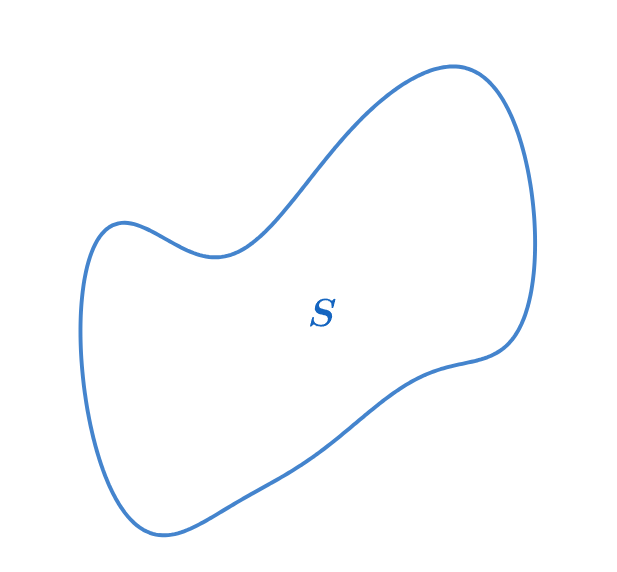
\includegraphics[height=7cm]{calculus/images/calculus_2024_02_07_0}
    \end{center}

    Надо найти ее площадь S

    Произведем ее дробление на маленькие элементарные фигуры, площадь которых мы можем посчитать:

    \begin{center}
        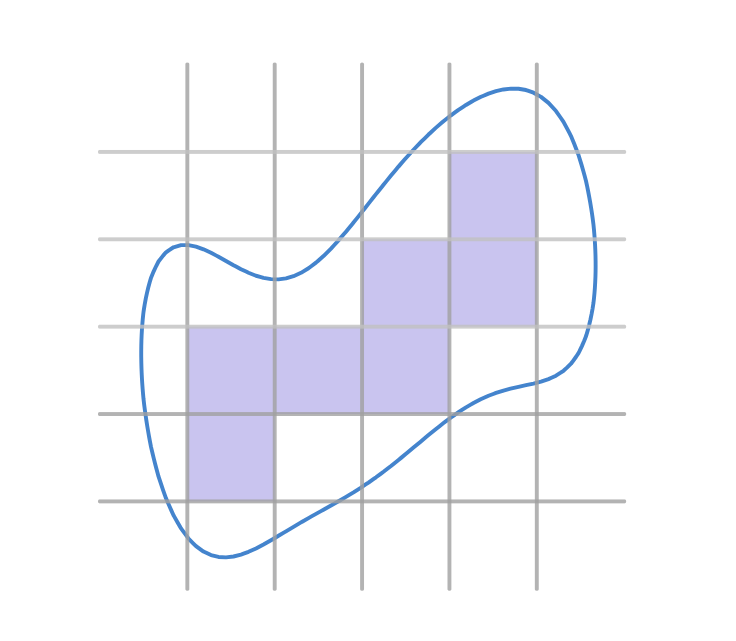
\includegraphics[height=7cm]{calculus/images/calculus_2024_02_07_1}
    \end{center}

    Уменьшаем дробление, чтобы свести погрешность к 0 (погрешность между истинной площадью и суммарной площадью прямоугольников)

    Сведем задачу к простейшей в ДПСК:

    \vspace{10mm}


    \begin{multicols}{2}
        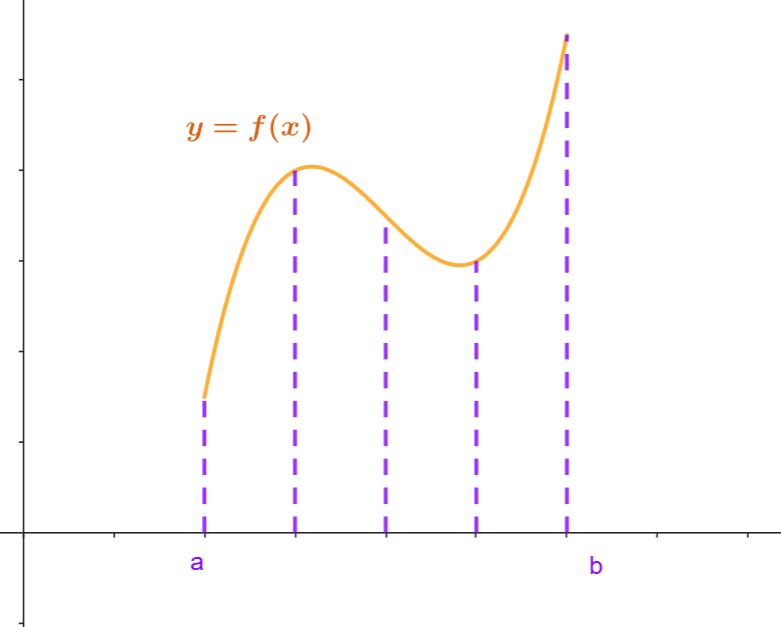
\includegraphics[height=6cm]{calculus/images/calculus_2024_02_07_2}

        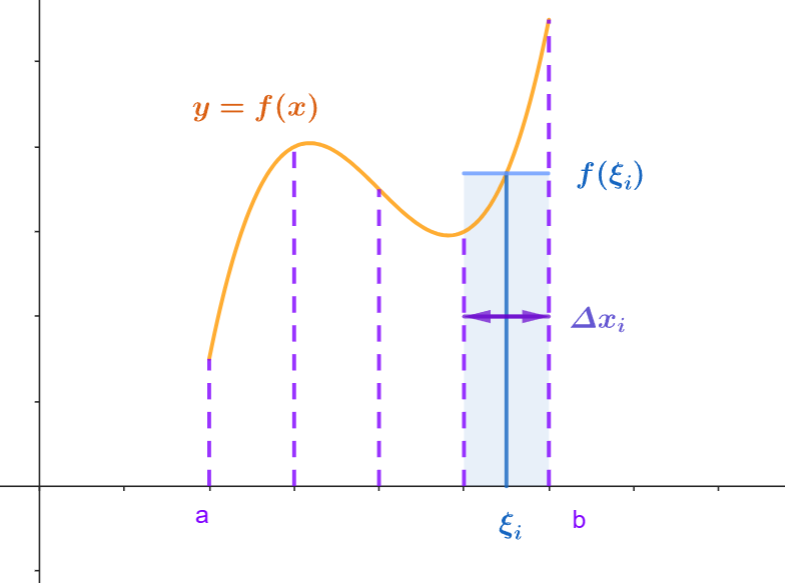
\includegraphics[height=6cm]{calculus/images/calculus_2024_02_07_3}
    \end{multicols}

    \begin{enumerate}
        \item Вводим разбиение отрезка $[a; b]\ (a < b)$ точками $a < x_0 < \dots < x_n < b$

        $T = \Set{x_i}^n_{i=0}$

        \item Выбираем средние точки на частичных отрезках $[x_{i-1}, x_i]^n_{i=1}$

        $\Set{\xi_i}_{i=1}^n$ - набор средних точек

        $\Delta x_i \stackrel{\text{обозн.}}{=} x_i - x_{i-1}$ - длина отрезка

        \item Строим элементарные прямоугольники
        \item Составляем сумму площадей всех таких прямоугольников:

        \[\sigma_n = \sum^n_{i=1} \Delta x_i f(\xi_i)\]

        - интегральная сумма Римана

        \item Заменяя разбиение, выбор $\xi_i$ при каждом $n$, получаем последовательность $\Set{\sigma_n}$

        При этом следим, чтобы ранг разбиения $\tau = \max\limits_{1 \leq i \leq n} \Delta x_i \rightarrow 0$ при $n \to \infty$

        Иначе получим неуничтожаемую погрешность

        \item \Def \hypertarget{integraldefinition}{Если существует конечный предел интегральной суммы} и он не зависит от типа,
        ранга дробления и выбора средних точек, то он называется определенным интегралом

        \[\lim_{\substack{n\to\infty \\ \tau\to0}} \sigma_n = \lim_{\substack{n\to\infty \\ \tau\to0}} \sum^n_{i=1} \Delta x_i f(\xi_i) \stackrel{\text{def}}{=} \int_a^b f(x)dx\]

    \end{enumerate}

    \Nota Независимость от дробления и выбора средних точек существенна

    \Ex $\mathcal{D} = \begin{cases}
                           1,\ x \in [0, 1], x \not\in \mathbb{Q} \\ 0,\ x \in [0, 1], x \in \mathbb{Q}
    \end{cases}$

    Сумма Римана для этой функции неопределенна, так как все зависит от выбора средних точек:
    \begin{itemize}
        \item если средние точки иррациональные, то сумма равна единице
        \item иначе сумма равна нулю
    \end{itemize}

    В обозначении определенного интеграла $a$ и $b$ называют нижним и верхним пределами интегрирования соответственно

    Дифференциал $dx$ имеет смысл $\Delta x$, понимается как б. м., то есть:

    $f(x) dx$ - площадь элементарных прямоугольников, тогда

    $\int^b_a f(x) dx$ - сумма этих прямоугольников

    \vspace{5mm}

    \begin{enumerate}
        \item $\int_a^a f(x)dx \stackrel{\text{def}}{=} 0$
        \item $\int_a^b f(x)dx = -\int_b^a f(x)dx$
    \end{enumerate}

    Можно доказать, что определенный интеграл существует для всякой непрерывной на отрезке функции

    \underline{Геом. смысл}: \hypertarget{integralgeommeaning}{Заметим, что в определении интеграл} - площадь подграфика функции $(f(x) \geq 0)$

    Заметим, что для $f(x) \leq 0 \quad \int_a^b f(x)dx = -S$


    \section{1.2. Свойства}
    \hypertarget{integralproperties}{}

    \begin{enumerate}
        \item Линейность пределов $\Longrightarrow$ линейность пределов

        $\lambda \int^b_a f(x)dx + \mu \int^b_a g(x)dx = \int^b_a (\lambda f(x) + \mu g(x)) dx \quad (\lambda, \mu \in \Real)$

        \item Аддитивность (часто для кусочно-непрерывных функций с конечным числом точек разбивается на участки непрерывности)

        $\int^b_a f(x)dx + \int^c_b f(x)dx = \int^c_a f(x)dx$

        Доказательства строятся на свойствах конечных сумм и пределов

        \item \hypertarget{integralevaluation}{Оценка определенного интеграла}

        $f(x)$ непрерывна на $[a; b]$ (имеет наимен. ($m$) и наибол. ($M$) значения). Тогда:

        $m (b-a) \leq \int^b_a f(x)dx \leq M(b - a)$

        $\Box$ Док-во:

        По теореме Вейерштрасса 2 $f(x)$ принимает наименьшее и наибольшее значения и для всякого $x$ из $[a; b]$:  $m <= f(x) <= M$

        Так как все средние точки принадлежат $[a; b]$, то

        $m \leq f(\xi_i) \leq M \quad \forall \xi_i$

        $m \Delta_i \leq f(\xi_i) \Delta_i \leq M \Delta_i$

        $m \sum_{i=1}^n \Delta x_i \leq f(\xi_i) \sum_{i=1}^n \Delta x_i \leq M \sum_{i=1}^n \Delta x_i$

        Предельный переход:

        $\lim_{\substack{n\to\infty \\ \tau\to0}} m \sum_{i=1}^n \Delta x_i \leq \int^b_a f(x) dx \leq \lim_{\substack{n\to\infty \\ \tau\to0}} M \sum_{i=1}^n \Delta x_i$

        $m \lim_{\substack{n\to\infty \\ \tau\to0}} \sum_{i=1}^n \Delta x_i \leq \int^b_a f(x) dx \leq M \lim_{\substack{n\to\infty \\ \tau\to0}} \sum_{i=1}^n \Delta x_i$

        $m (b - a) \leq \int^b_a f(x) dx \leq M (b - a)$

        $\Box$


        \item \Th \hypertarget{theoremlagrangeaboutaverage}{Лагранжа о среднем} (в интегральной форме)

        $f(x) \in C^\prime_{[a,b]} \Longrightarrow \exists \xi \in (a, b) \ f^\prime(\xi) = \frac{f(b) - f(a)}{b - a}$

        Тогда найдется такая средняя точка, что

        $f(x) \in C_{[a,b]} \Longrightarrow \exists \xi \in (a, b) \ f(\xi)(b - a) = \int^b_a f(x)dx$

        % help me

        $\Box$

        $m \leq \underset{\text{некоторое число}}{\undergroup{\frac{1}{b-a} \int_a^b f(x)dx}} \leq M$ по свойству выше

        По теореме Больцано-Коши $f(x)$ непрерывна, поэтому пробегает все значения от $m$ до $M$

        Значит найдется такая точка $\xi$, что $f(\xi) = \frac{1}{b-a} \int_a^b f(x)dx$

        $\Box$

        \item Сравнение интегралов

        $f(x), g(x) \in C_{[a, b]} \quad \forall x \in [a, b] \quad f(x) \geq g(x)$

        Тогда $\int_a^b f(x)dx \geq \int_a^b g(x)dx$

        $\Box$

        $\int_a^b f(x)dx - \int_a^b g(x)dx = \int_a^b (f(x) - g(x))dx =
        \lim_{\substack{n\to\infty \\ \tau\to0}} \sum_{i=1}^n \underset{\geq 0}{\undergroup{(f(\xi_i) - g(\xi_i))}} \underset{\geq 0}{\undergroup{\Delta x_i}} \geq 0$

        $\Box$


        \item Интеграл и модуль

        $\left| \int^b_a f(x)dx \right| \leq \int^b_a |f(x)| dx$

        $\Box$

        $\int^b_a f(x)dx = \lim_{\substack{n\to\infty \\ \tau\to0}} \sum_{i=1}^n f(\xi_i) \Delta x_i = \lim_{n\to\infty} \sigma_n$

        $\int^b_a |f(x)|dx = \lim_{\substack{n\to\infty \\ \tau\to0}} \sum_{i=1}^n |f(\xi_i)| \Delta x_i$

        Докажем, что $\lim_{n\to\infty} |\sigma_n| = |\lim_{n\to\infty} \sigma_n|$

        Так как определен $\int^b_a f(x)dx = \lim_{n\to\infty} \sigma_n = S \in \Real$, то можно рассмотреть случаи

        $S > 0: \quad \exists n_0 \ \forall n > n_0 \ \sigma_n > 0$ (вблизи $S$)

        $\lim_{n\to\infty} |\sigma_n| = |\lim_{n\to\infty} \sigma_n|$

        $S > 0: \quad \exists n_0 \ \forall n > n_0 \ \sigma_n < 0$ (вблизи $S$)

        $\lim_{n\to\infty} |\sigma_n| = -\lim_{n\to\infty} \sigma_n = |\lim_{n\to\infty} \sigma_n|$

        $S = 0: \lim_{n\to\infty} |\sigma_n| = |\lim_{n\to\infty} \sigma_n| = 0$

        $\left| \int^b_a f(x)dx \left| = |\lim_{n\to\infty} \sigma_n| = \lim_{n\to\infty} |\sigma_n| =
        \lim_{\substack{n\to\infty \\ \tau\to0}} \left|\sum_{i=1}^n f(\xi_i) \Delta x_i\right| \leq \lim_{\substack{n\to\infty \\ \tau\to0}} \sum_{i=1}^n |f(\xi_i)| \Delta x_i$ (модуль суммы меньше или равен сумме модулей)

        $\Box$

    \end{enumerate}

    \Nota Интеграл и разрыв

    Изъятие из отрезка не более, чем счетного числа точек, не меняет значение интеграла, что позволяет считать интеграл на интервале

    \Nota Сходимость интеграла - в определении интеграла подчеркивается, что это число.
    Если предел интегральных сумм не существует или бесконечен, говорят, что интеграл расходится

    \Nota Вычисления

    Определение дает способ вычисления и его можно упростить:

    $\forall i\ \Delta x_i = \Delta x, \quad \xi_i = \begin{sqcases}
                                                         x_{i-1} \\ x_i
    \end{sqcases}$ - концы отрезка

    Так вычисляют \enquote{неберущиеся интегралы}

    Для функций, у которых первообразные выражаются в элементарных функциях используется не этот метод, а формула Ньютона-Лейбница


    \section{1.3. Вычисление определенного интеграла}


    \section{1.3.1. Интеграл с переменным верхним пределом}
    \hypertarget{integralwithvariableupperlimit}{}

    Дана $f(x): [a; +\infty), f(x) \in C_{[a; +\infty)}$

    $\forall x \in [a; +\infty)$ определен $\int^x_a f(x) dx$

    Таким образом определена функция $S(x) = \int_a^x f(x)dx$ - переменная площадь

    В общем случае обозначим $\Phi(x) = \int^x_a f(t) dt \quad t \in [a, x]$

    Итак, различают три объекта:

    \begin{enumerate}
        \item Семейство функций: $\int f(x) dx = F(x) + C$
        \item Функция $\int^x_a f(t) dt = \Phi(x)$
        \item Число $\int^b_a f(x) dx = \lambda \in \Real$
    \end{enumerate}

    Выявим связь между ними.

    \Th \hypertarget{theorembarrow}{Об интеграле с переменным верхним пределом} (Барроу)

    $f(x) : [a;+\infty) \to \Real \quad f(x) \in C_{[a;+\infty+}$

    Тогда $\Phi(x) = \int^x_a f(t) dt$ - первообразная для $f(x)$ - $\Phi(x) = F(x)$

    $\Box$

    Докажем по определению

    $\Phi^\prime(x) = \lim_{\Delta x \to 0}\frac{\Delta \Phi}{\Delta x} = \lim_{\Delta x \to 0}\frac{\Phi(x + \Delta x) - \Phi(x)}{\Delta x} =
    \lim_{\Delta x \to 0}\frac{\int^{x + \Delta x}_a f(t)dt - \int^{x}_a f(t)dt}{\Delta x} =
    \lim_{\Delta x \to 0}\frac{\int^{x + \Delta x}_x f(t)dt}{\Delta x} = [\text{по \Ths Лагранжа } \exists \xi \in [x;x + \Delta x]] =
    \lim_{\Delta x \to 0} \frac{f(\xi)\Delta x}{\Delta x} = \lim_{\substack{\Delta x \to 0 \\ \xi \to x}} f(\xi) = f(x)$

    $\Box$

    \Th \hypertarget{formulanewtonleibniz}{Основная теорема математического анализа} (формула Ньютона-Лейбница, N-L)

    $f(x) \in C_{[a;b]}, F(x)$ - какая-либо первообразная $f(x)$

    \fbox{$\int^b_a f(x)dx = F(x) \Big|^b_a = F(b) - F(a)$}

    $\Box$

    Для $f(x)$ определена $\Phi(x) = \int_a^x f(t)dt = F(x) + C$

    Найдем значения $\Phi(a)$ и $\Phi(b)$

    $\Phi(a) = F(a) + C = \int^a_a f(t)dt = 0 \Longrightarrow F(a) + C = 0 \Longrightarrow F(a) = -C$

    $\Phi(b) = F(b) + C = F(b) - F(a) = \int^b_a f(t) dt$

    $\int^b_a f(x)dx = F(b) - F(a)$

    $\Box$


    \section{1.3.2. Методы интегрирования}

    1* \hypertarget{integralsubstitution}{Замена переменной в определенном интеграле}

    \Th $f(x) \in C_{[a;b]} \quad x = \varphi(t) \in C^\prime_{[\alpha;\beta]}, \varphi(\alpha) = a, \varphi(\beta) = b$

    $\int^b_a f(x)dx = \int^\beta_\alpha f(\varphi(t)) \varphi^\prime(t) dt$

    $\Box$

    N-L: $\int^b_a f(x)dx = F(x) \Big|_a^b$

    Докажем, что $F(x) = F(\varphi(t))$ - первообразная для $f(\varphi(t))\varphi^\prime(t)$

    $\frac{dF(\varphi(t))}{dt} = F^\prime(\varphi(t)) \varphi^\prime(t)$

    $\frac{dF(\varphi(t))}{d\varphi(t)}\frac{d\varphi(t)}{dt} = \frac{dF(x)}{dx} \varphi^\prime(t) = f(x)\varphi^\prime(t)$

    $\Box$

    \Ex $\int_0^{\frac{1}{2}} \frac{dx}{\sqrt{1 - x^2}} = \begin{bmatrix}
                                                              x = \sin t \\ x \uparrow^\frac{1}{2}_0 \ t \uparrow_0^\frac{\pi}{6}
    \end{bmatrix} =
    \int_0^\frac{\pi}{6} \frac{dt}{\sqrt{1 - \sin^2 t}}\cos t =
    \int_0^\frac{\pi}{6} \frac{dt}{|\cos t|} \cos t = \int_0^\frac{\pi}{6} dt = t \Big|_0^\frac{\pi}{6} = \frac{\pi}{6}$

    2* \hypertarget{integralbyparts}{По частям}

    \Th $u, v \in C^\prime_{[a;b]} \quad uv \Big|_a^b = u(b)v(b) - u(a)v(a)$

    Тогда: $\int^b_a udv = uv \Big|_a^b - \int^b_a vdu$

    $\Box$

    $u(x)v(x)$ - первообразная для $u^\prime(x)v(x) + v^\prime(x)u(x)$

    Или $d(uv) = udv + vdu$

    По формуле N-L $\int_a^b (udv + vdu) = \int^b_a d(uv) = u(x)v(x) \Big|^b_a$

    $\int_a^b udv = uv \Big|^b_a - \int^b_a vdu$

    $\Box$

    \Ex $\int_1^e \ln x dx = x \ln x \Big|^e_1 - \int^e_1 xd\ln x = e \ln e - 1 \ln 1 -
    \int^e_1 dx = e - x \Big|_1^e = 1$

    \Nota Не всякий интеграл вида $\int^b_a f(x) dx $ является определенным

    \Ex $\int^e_0 \ln x dx = x \ln x \Big|_0^e - x \Big|_0^e = e \ln e - \underset{0 \cdot \infty}{\undergroup{0 \ln 0}} - e$ - несобственный интеграл


\end{document}
